\chapter{Fabrication of Microcavity on Silica}
\label{chap:fabrication}
%Descrição do processo de fabricação. Aqui eu não tenho certeza o quanto vai ser aprofundado.  
One of the must desirable characteristics of a optical microcavity is the capacity of confine light for many cycles, there are two way to reach this characteristic, one is decrease the round trip time and the decrease the intrinsic losses. the round trip time is directly correlated with the geometry of the microcavity, as we work with a fixed geometry our goal is to decrease the intrinsic losses, which is analogous to increase the quality factor. 

The intrinsic losses are defined as the loss of energy for any other channel that is not the source. We have basically sort of losses: scattering, absorption and band loss~\needcit. As or cavity have a relatively large radius the band loss is negligible~\needcit. The optical absorption of the silica, both in visible and infrared, are considerable low, so that the limiting of the quality factor is the scattering loss. 

A typical microfabrication process consists of three main steps: lithography, etching and release. Often this process, specially lithography and etching, introduce some blemishes in the device, we seek a form to smooth this defects.
Toroidal microcavities, for example, use a reflow process by heating the surface of the device close to melt temperature making the surface tension reconstruct the surface smoother~\needcit, however, the reflow smoothing is difficult to be applied in larger cavities and limits the integrability of the device. Another option to reach this goal is use a chemical etch~\needcit leading to the wedge shape devices. 

A more technical step-by-step recipe is present in the Appendix~\ref{app:fabric}, in this Chapter we shall look for the details and result of each of the main steps.

\section{Overview}

The Fig.~\ref{fig:fab_step} shows the result of each step of the fabrication process. Our fabrication process begin with a silicon wafer of some inches, typically 4'', with a oxidized layer with 3~$\mu$m of thickness \textbf{(I)}. We divided it in 1$\times$1 mm shards, each shard is a sample. Initially the sample is cleaned using a organic cleaning with Trichloroethylene, isopropyl alcohol, acetone and water, all in a ultrasonic cleaner. The ultrasonic cleaner is also used to deposited the adhesion promoter (SurPass\regmark~3000). The Resist is deposited in a spinner at 4000 RPM, we use a positive photoresit (Sc1827) exposed to a UV using a mask aligner (KARL SUSS MJB3) and developed with a solution of three parts of water for one part of developer (AZ\regmark 351) \textbf{(II)}. Before the exposure the sample is soft baked at 110$^o$C for 1 minute and after the sample is heat at 130$^o$C for 5 minutes to reflow the resist\textbf{(III)}. The silicon oxide layer is etched using a buffered solution of hydrofluoric acid for 40 minutes, giving rise to the wedge disk\textbf{(IV)}. Lastly, the sample is etched with tetramethylammonium hydroxide (TMAH)\textbf{(V)}. 

\begin{figure}[!t]
    \centering
    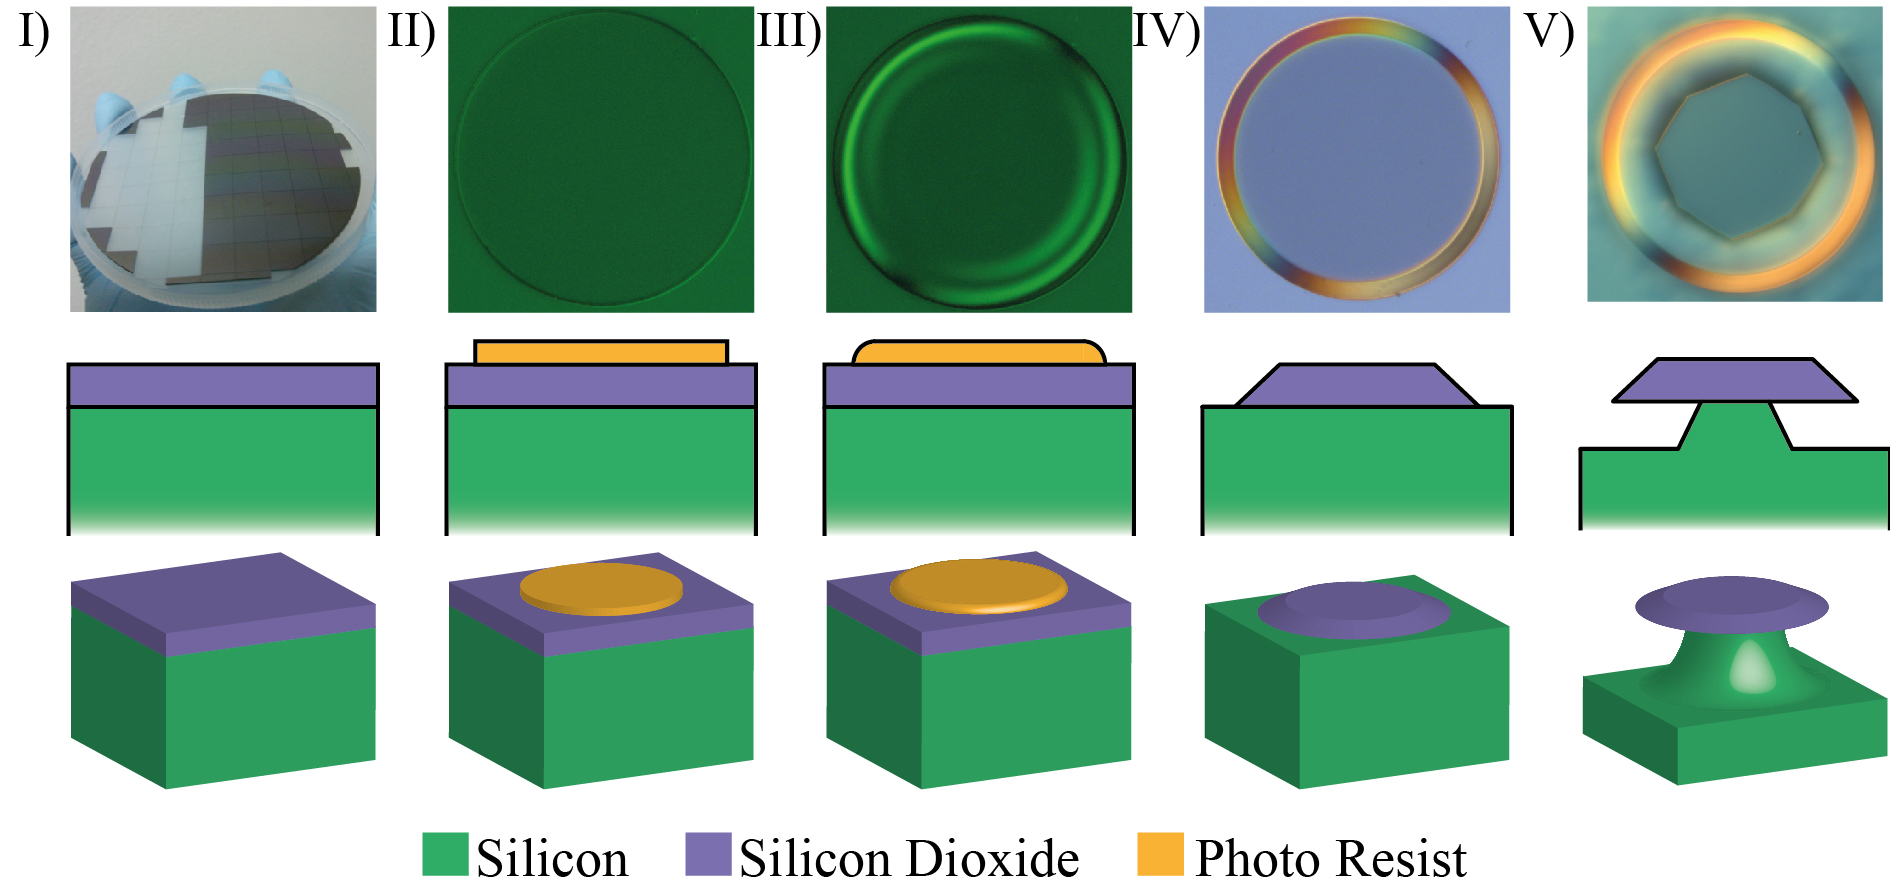
\includegraphics[width = 16cm]{figuras/Dissertation_fabrication_steps.jpg}
    \caption{\textbf{Steps of Fabrication:} The first row shows pictures taken in a optical microscopy. The second row shows a schematic draw of the layers. The last row show a perspective scheme.}
    \label{fig:fab_step}
\end{figure}

\section{Lithography}

In top-down microfabrication it is usually applied to transfer a pattern to a mask in order to protect the subtract during the etching process. 
\begin{figure}[!h]
    \centering
    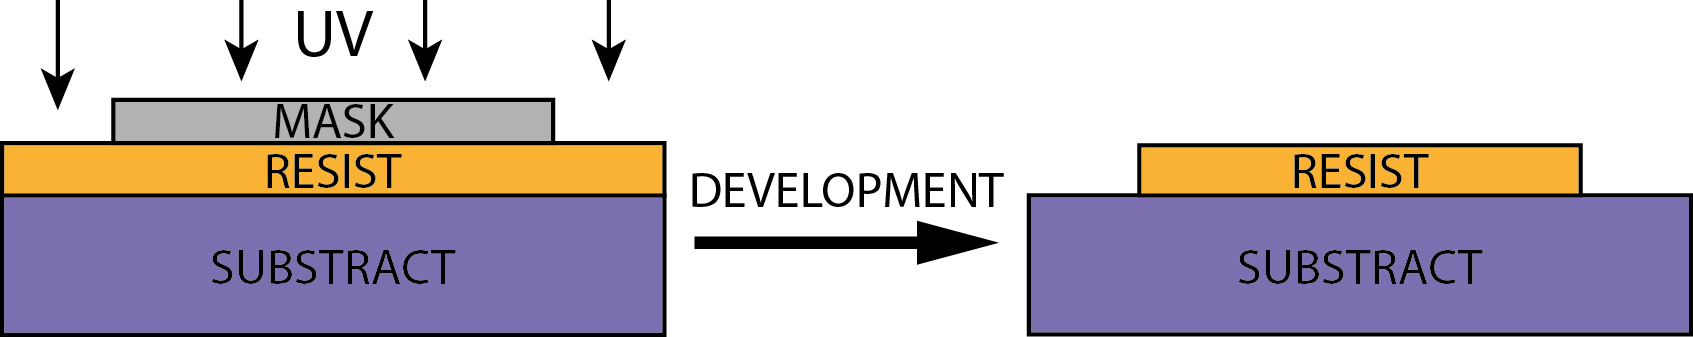
\includegraphics[width = 16cm]{figuras/Dissertation_litho.jpg}
    \caption{\textbf{Contact lithography}: A chrome mask is contacted with the resist and physically block the UV radiation, enabling to sensitize selectively and to transfer the mask pattern to the resist.}
    \label{fig:litho}
\end{figure}

Initially we deposit a photo sensitive resin, called resist. A chrome mask with the device pattern is used to cover-up the resist, then a UV light source is used to expose the uncovered resist, as schematically showed in Fig~\ref{fig:litho}. The UV light cause a chemical change in the resist that allows it to be removed using a specific solution, called developer. 

A crucial aspect in the lithography process is the adherence between the resist and the substrate. To fabricate this cavities we use a wet etching process, as we shall see below, which is very affected by the adherence. The Fig.~\ref{fig:adhrence_problem} 
shows the result of a etching with poor adherence, em some case the device totally vanish from the sample, and the process is not reproducible.
\begin{figure}[!hbt]
    \centering
    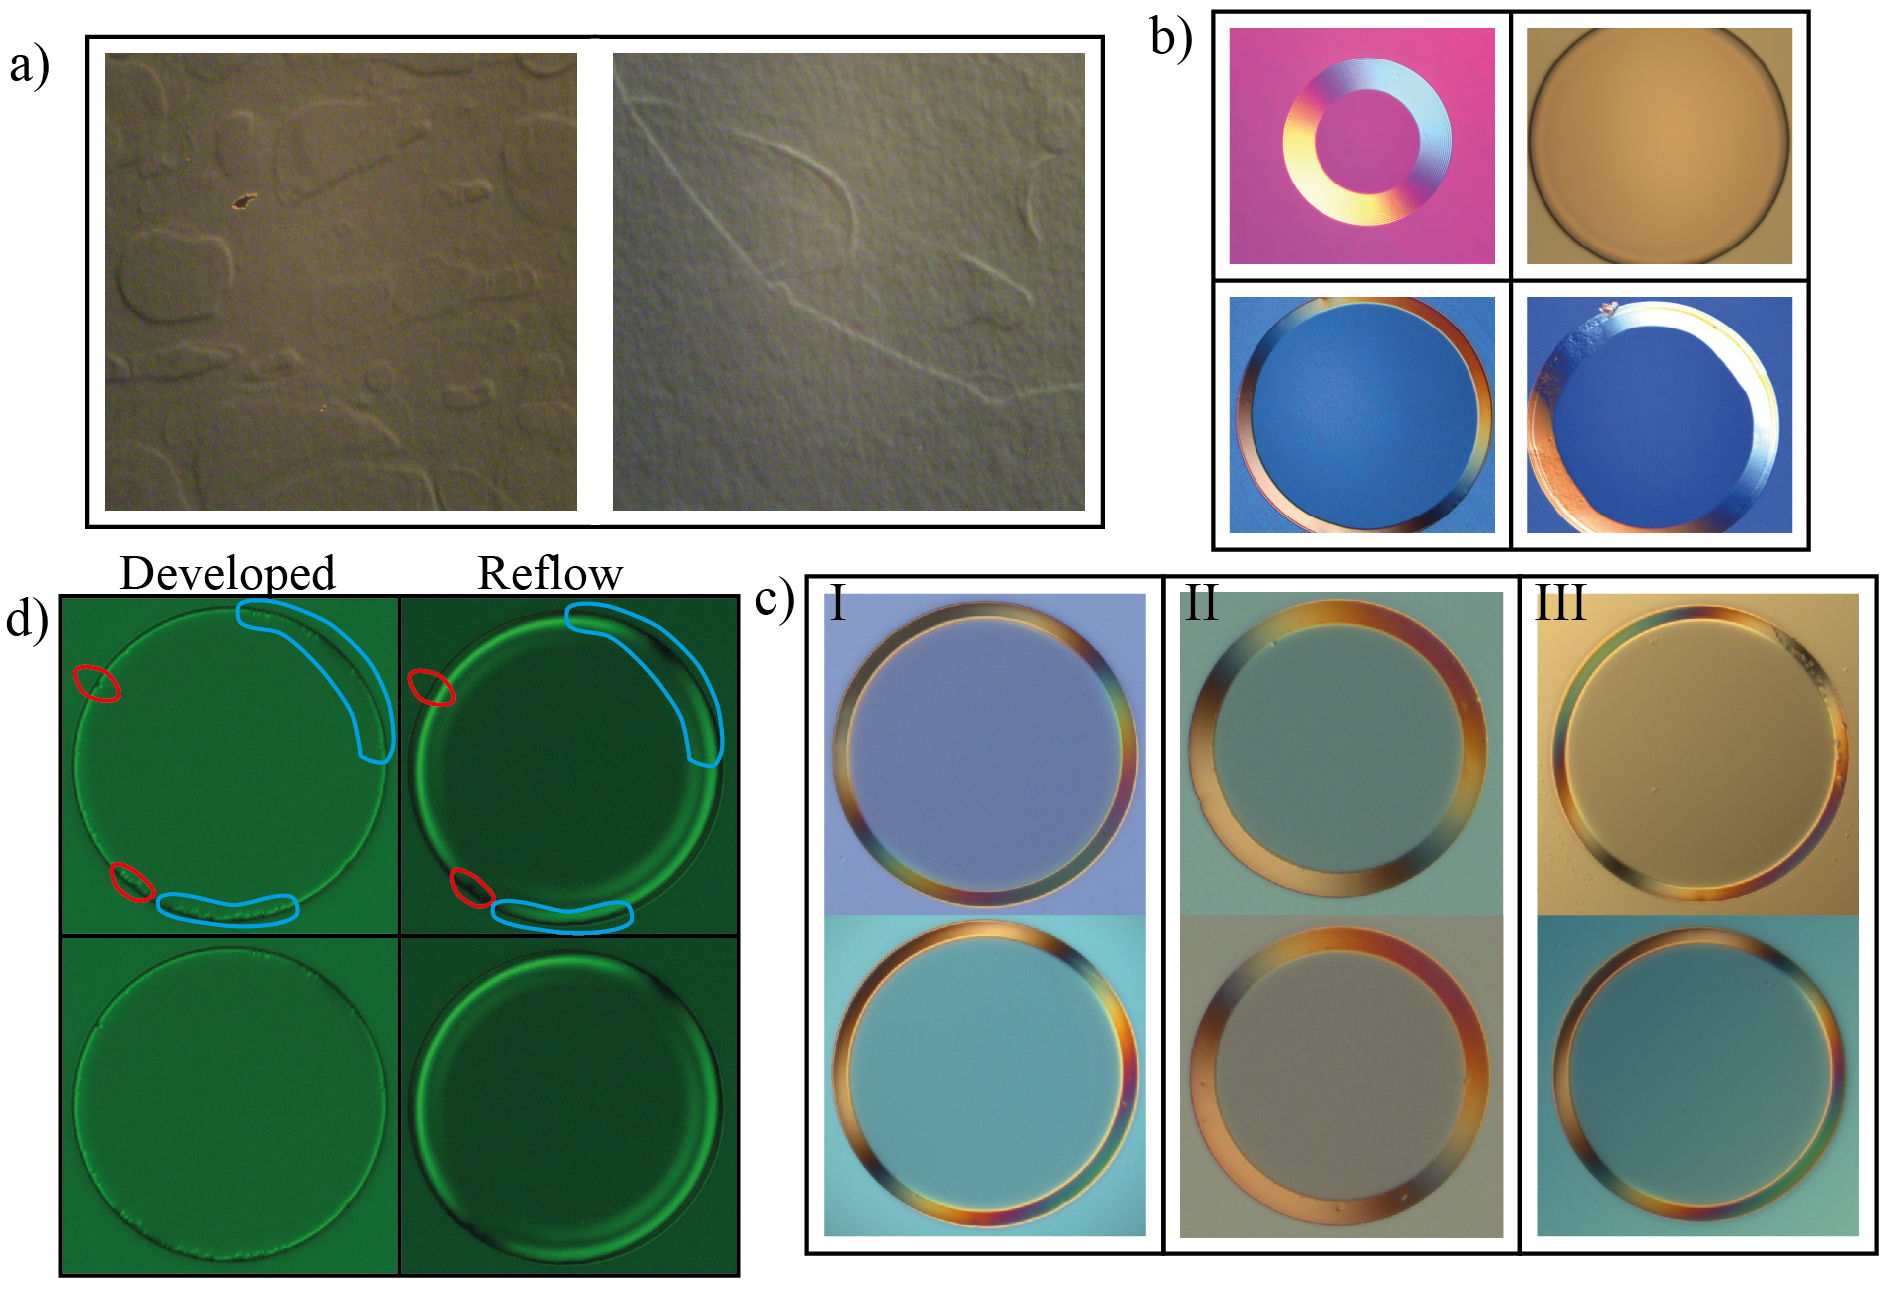
\includegraphics[width = 16cm]{figuras/Dissertation_etching_result.jpg}
    \caption{\textbf{a) Substrate Defect:} The irregularity in the surface of the substrate prevent a good adherence of the resist. \textbf{Comparison of Reproducibility: b)} Examples of different samples made with the same recipe using the commercial wafer; due to limitation on the optical microscopy, isn't possible to use a scale, however all images was made using the same magnification. \textbf{c)} Examples of different samples using the non-commercial wafer; each par of images was made using the same recipe, it shows that the result is consistent. \textbf{d) Reflow:}(top) Highlighted in blue defects suppressed by the reflow, in red defects that remains after the reflow. (bottom) Picture of the same cavity without the highlight to ease visualization.}
    \label{fig:adhrence_problem}
\end{figure}

In order to improve the adherence of the resist there are some cares that should be taken before the resist deposition. We have notice that the commercial wafer initially used as substrate present some irregularity in the surface, as show in Fig.~\subref{fig:adhrence_problem}{a}, this defects lead to a poor adherence and problems cited above. To solved it we used a non-commercial wafer grown by wet-oxidation. The reproducibility of the process presented a significant improvement, which can be seen in the comparation of the Fig.~\subref{fig:adhrence_problem}{b}. Besides that, a non aggressive organic cleaning is necessary to archive the good results presented.

The replication of the mask pattern in the resist after the development is highly accurate, which could be a problem since it will replicate the defects in the mask also, as can be easily spotted in Fig. A technique to attenuate this kind of defect is to heat the sample to the softening temperature of the resist, in this way the borders of the resist will reconstruct smoother~\needcit, this technique is called reflow. The result is shown in the Fig.~\subref{fig:adhrence_problem}{c}.

With a well deposited kinkiless resist we can etch the sample to fabricate the wedge disk cavities. 

\section{Etching}

In typical etching process, the resist act as a etch shield protecting the subtract from the etch. In this process, however, the resist orientate the etch direction by smoothly peel off during the etching. The Fig.~\ref{fig:wedeg_grow} illustrate how it occurs. Lets say, taking some linguistic liberty, that the interface between the solution and the silica act as a "etch source" of a spherical "etching wave". The "etch wavefront" appears under the resist, centered at the lower edge, when the etchant infiltrates between the resist, it peels off and a new "etch source" is created. A continuous adiabatic resist peeling leads to a straight wall with shallow wedge angle. %The result of a inhomogeneous resist peeling is showed in the Fig~\ref{fig:ethc_wrong}. 

\begin{figure}[!ht]
    \centering
    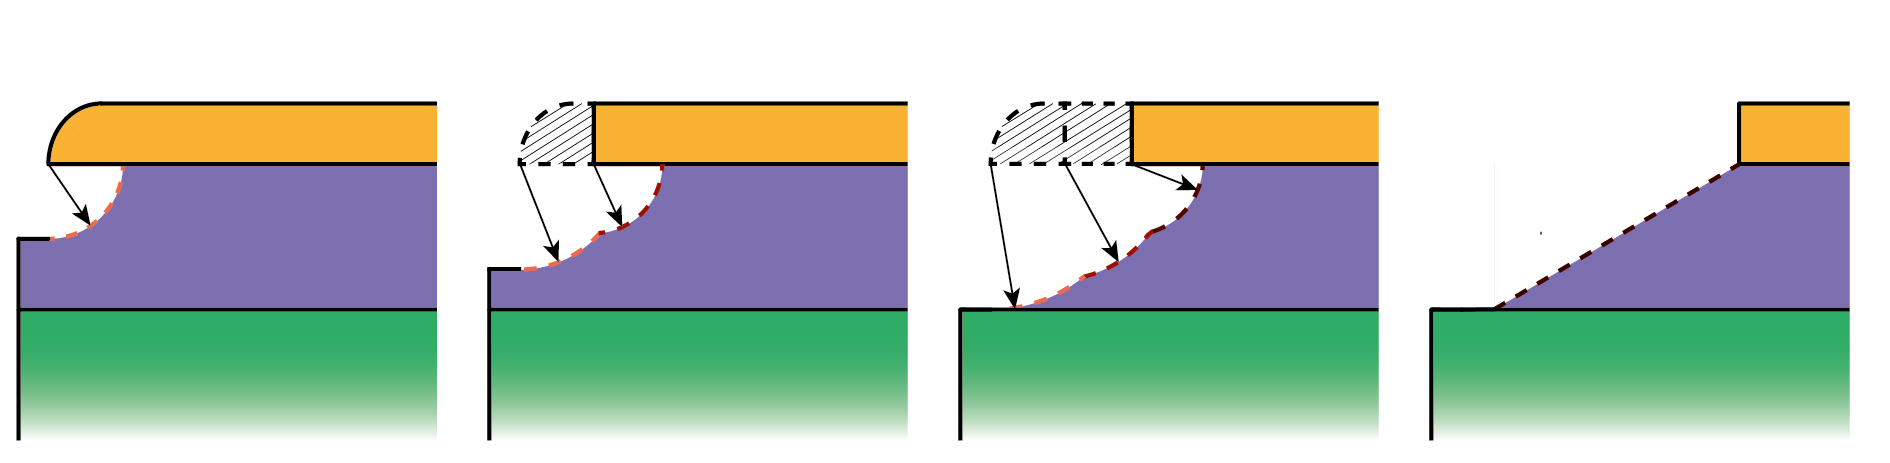
\includegraphics[width = 16cm]{figuras/Dissertation_etching.jpg}
    \caption{\textbf{Peeling Process Pictured:} The resist keep pilling off as long the sample is keeping in the etchant solution. A continuous process with small steps lead to a well defined wedge.}
    \label{fig:wedeg_grow}
\end{figure}

The reaction between the silica and the hydrofluoric acid occurs following the equation~\cite{Kang_2002} 
\cheeq{SiO2 + 4HF -> SiF4$_{(g)}$ + 2H2O}.
A buffered solution is used to maintain the solution concentration constant and decrease the etch rate, leading to a slower reaction which suppress the occurrence of abrupt defects contributing to a smooth surface, decreasing the scattering loss and enabling high Q cavities. However, a scanning electronic microscopy show unexpected defects in the cavities surface, as shows Fig.\subref{fig:ethc_wrong}{a}. This image was made using the initial commercial wafer, due to lack of time it wasn't possible to check if the new wafer solved this problem, thus, the origin of this problem is still unknown. 

Another common defect after the etching process is the rise of holes, especially in the wedge region. It is probable that the pressure between the mask and the resist in the contact lithography step creates microcracks that allow the etchant to infiltrate through the resist and etch the silica faster in this points, as pictured in Fig~\subref{fig:ethc_wrong}{b}, however a more detailed study would be necessary to prove this hypothesis. 

\begin{figure}[!ht]
    \centering
    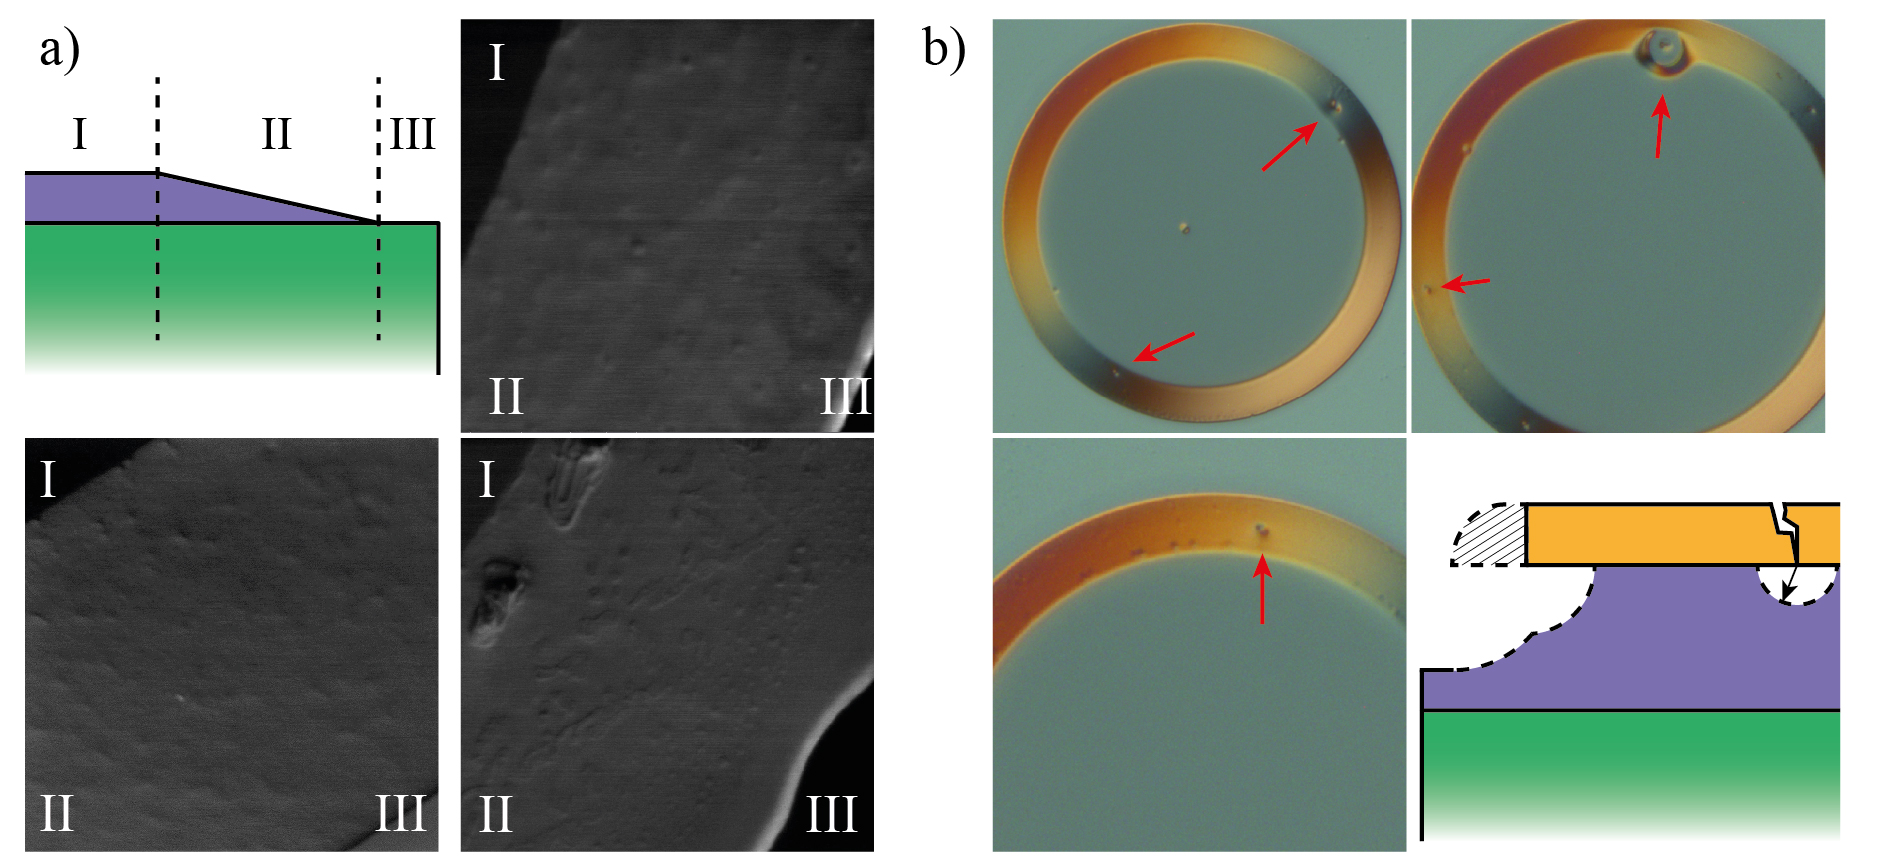
\includegraphics[width = 16cm]{figuras/Dissertation_etchin_def.jpg}
    \caption{\textbf{After Etching Defects:a)} Roughness at wedge surface. \textbf{b)} holes in the devices probable originated from micro cracks}
    \label{fig:ethc_wrong}
\end{figure}

The etching step build up the device, however they are fully in touch with the silicon layer. To improve the index contrast and enable the mode to be confined, we must release the cavity from the substrate, which is made by etching the silicon.

\section{Release}

The release procedure usually is made using a isotropic etch, otherwise the device would act as a mask. However, due to the crystalline characteristic of the silicon it is possible to apply a anisotropic etch, since the preferential direction is the atomic plan that goes under the device, leading to polygonal pedestal as can be seen in Fig~\subref{fig:release}{a}I and II.

The wet etch of the silicon occurs at presence of hydroxide that react with the silicon according with the reaction
\cheeq{Si + 2OH- + 2H2O -> Si (OH4)- + H2$_{(g)}$}
which is preferentially occurs at the (111) plane direction~\cite{Glembocki_1985}, enabling the releasing of the devices. For that we have test the etch using potassium hydroxide (KOH) and tetramethylammonium hydroxide (TMAH).

The compound \ce{Si(OH)4}, named orthosilicic acid, is aqueous and can also be obtained by the reaction\cite{madou2002fundamentals} 
\cheeq{SiO2 + 2H2O <=> Si(OH)4}
which mean that the etching of the silicon can also affect the silicon oxide device. In order to increase the selectivity of the process we have to adjust the concentration and temperature parameters of the solution~\needcit 

\begin{figure}[!b]
    \centering
    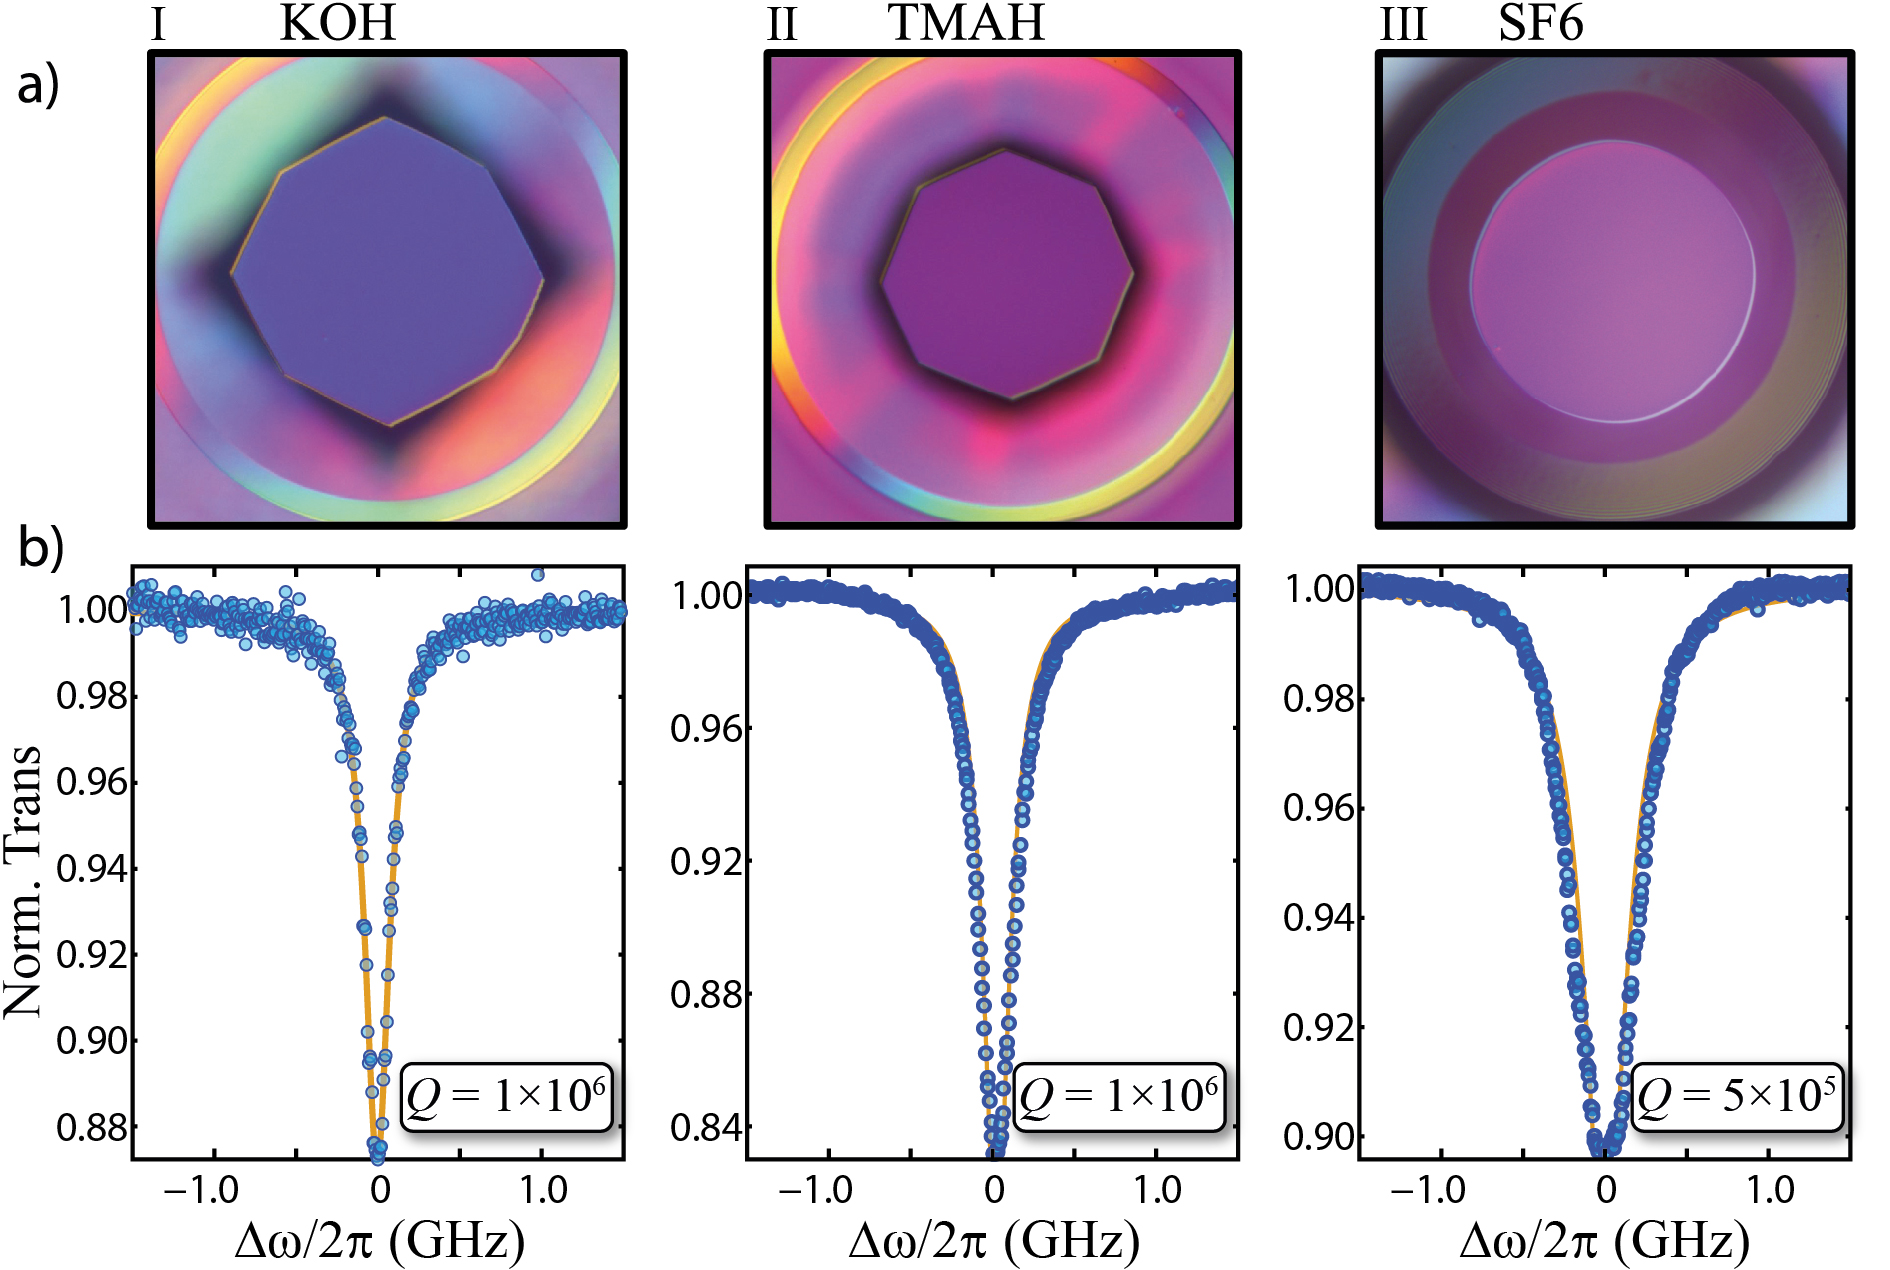
\includegraphics[width = 16cm]{figuras/Dissertation_release.jpg}
    \caption{\textbf{Release Process Comparation:a)} The initial difference between the anisotropic, KOH and THMA, and the isotropic release lies in the pedestal shape, that can introduce stress in the device surface, hence, introduce losses. \textbf{b)} To analyse the effect of the release in the losses, it was measured the maximum Q factor reached, the result don't show a considerable variation.}
    \label{fig:release}
\end{figure}
The polygonal shape of the pedestal could be introducing mechanical stress in the interface between the silica and the silicon, with would lead to a increase in the losses. In order to test this hypotheses a isotropic release process was test. The cavities was released by dry etch, using \ce{SF6}/\ce{O2} plasma~\cite{Eisele_1981}, leading to a pedestal as show in Fig~\subref{fig:release}{a}III. In the etch process we have, basically, two reaction occurring
\begin{subequations}
    \begin{alignat}{2}
        &\ce{Si + 4F& & -> SiF4}\label{etc:si}\\
        &\ce{SiO2 + 4F& & -> SiF4 + O2}\label{etc:sio}.
    \end{alignat}
\end{subequations}
However, the reaction probability to the reaction~\ref{etc:sio} is much lower than that of the reaction~\ref{etc:si}~\cite{Knizikevicius_2009}. The rigth set of parameters can lead to a high selective etching~\cite{Frederico_2003}. 
%https://www.sciencedirect.com/science/article/pii/S0921510797002171
 
The motivation for try different etching process is to determine what one causes less impact in the devices, once, was showed, all of then also etch silicon oxide. The result of each one is presented in the Fig. 

The parameter used to classify the cavities was the max reached Q factor. None of the process presented a high improvement. The Fig~\subref{fig:release}{b} brings the transmission for the mode with maximum Q factor. However, this test was done before we discovery the defects in the commercial wafer, in such way that the Q factor could already by limited early in the process. Due to practicality and reproducibility, we choose to do the release using TMAH.   
 
\section{Conclusion}

We found the main source of defects in or process, it was the defective commercial wafer, unfortunately it was found in a late stage of the project and it wasn't possible to revisited the other steeps to improve the fabrication results. 

It was possible to elaborate a fully reproducible recipe to fabricate wedge micro cavities in silicon dioxide at in-house facilities. We identified the key point of each step leading to a list of problems that need to be solved;
\begin{itemize}
    \item Lithography
    \begin{itemize}
        \item[$\ast$] Defects in the chrome mask is replicated in the resist, is required to fabricate a mask with least defect as possible. 
        \item[$\ast$] The pressure necessary to contact photolythography possible create micro cracks that allow the resist to infiltrate between the resist, damaging the device.
    \end{itemize}
 
    \item Etching
    \begin{itemize}    
        \item[$\ast$] The result after the etching must be checked using SEM.
    \end{itemize}
    
    \item Release
    \begin{itemize}
        \item[$\ast$] The comparation between release techniques should be redone.
    \end{itemize}
\end{itemize}

Follow this list may determine the way to improve our fabrication process till the state of art~\needcit. 




